\documentclass[a4paper,11pt]{article}

\usepackage[english]{babel}
%\usepackage[portuguese]{babel}
\usepackage[T1]{fontenc}
\usepackage{amsmath, amssymb}
\usepackage{cancel}
\usepackage{graphicx}
\usepackage{color}
\usepackage{listings}

%%% To insert the code, you can use \begin{lstlisting} ...  \end{lstlisting}
\lstset{
    backgroundcolor=\color[rgb]{0.86,0.88,0.93},
    language=R, keywordstyle=\color[rgb]{0,0,1},
    basicstyle=\footnotesize \ttfamily,breaklines=true,
    escapeinside={\%*}{*)}
}

\begin{document}

%%%%%%%%%% Headings page %%%%%%%%%%%
\begin{figure}[!h] 
\includegraphics [scale=0.3] {Course_logo} \end{figure}
%\pagestyle{empty}
{\Large \noindent \bf Homework I}\\
 
\noindent {\Large \bf Student Name}
\\ Caio Cid Santiago Barbosa - 378596
\vskip0.8cm

%%%%%%%%%% Content starts here %%%%%%%%%%%
\section*{Exercise 1} 
Find the inverse Laplace transform by hand calculations of the following:
\begin{enumerate}
\item $F_1(s)=\cfrac{s-10}{(s+2)(s+5)}$ 
\item $F_2(s)=\cfrac{100}{(s+1)(s^2+4s+13)}$ 
\item $F_3(s)=\cfrac{s+18}{s(s+3)^2}$ 
\end{enumerate}

\noindent  Verify your results using the Symbolic toolbox in Matlab/Octave.\\

%\subsection*{Solution 1}

%%% To insert the code, you can use \begin{lstlisting} ...  \end{lstlisting}
%% To insert your plots, you can use 
% \begin{figure}[!h]  \includegraphics [scale=0.4] {Figures/myfilename} \end{figure}

\subsection*{Solution 1}
\begin{enumerate}
	\item $F_1(s)=\cfrac{s-10}{(s+2)(s+5)}\rightarrow F_1(s)=\cfrac{A}{s+2}+\cfrac{B}{s+5}$
	\begin{itemize}
		\item $ A = \lim\limits_{s\to-2}\cfrac{s-10}{s+5} = -4$
		\item $ B = \lim\limits_{s\to-5}\cfrac{s-10}{s+2} = 5$
	\end{itemize}
	$F_1(s)=\cfrac{-4}{s+2}+\cfrac{5}{s+5}
	\overset{\mathcal{L}^{-1}}{\longrightarrow}
	f_1(t)=5e^{-5t}-4e^{-2t}$
	\begin{lstlisting}
	syms s
	F(s) = (s - 10)/((s+2)*(s+5))
	ilaplace(F)
	
	ans =
	
	5*exp(-5*t) - 4*exp(-2*t)
	\end{lstlisting}
	\item $F_2(s)=\cfrac{100}{(s+1)(s^2+4s+13)}\rightarrow
	F_2(s)=\cfrac{A}{s+1}+\cfrac{Bs+C}{s^2+4s+13}$
	\begin{itemize}
		\item $ A= \lim\limits_{s\to-1}\cfrac{100}{s^2+4s+13}=10$
		\item $ F_2(s)=\cfrac{100}{(s+1)(s^2+4s+13)} =\cfrac{10}{s+1}+\cfrac{Bs+C}{s^2+4s+3}$
		\vskip0.4cm $\cfrac{100}{\cancel{(s+1)(s^2+4s+13)}}=\cfrac{(10+B)s^2+(B+C+40)s+130+C}{\cancel{(s+1)(s^2+4s+13)}}$
		\vskip0.4cm
		 $10+B=0\rightarrow B=-10$ 
		 \\$130+C=100\rightarrow C=-30$
		 \vskip0.4cm
		 $F_2(s)=\cfrac{10}{s+1}-\cfrac{10s+30}{s^2+4s+13}$
		 \vskip0.4cm
		 \item Sabendo que:
		 \\$\mathcal{L}(Ae^{-at}\cos(wt))=\cfrac{A(s+a)}{(s+a)^2+w^2}$
		 \hspace{0.2cm} e 
		 \\$\mathcal{L}(Be^{-at}\sin(wt))=\cfrac{Bw}{(s+a)^2+w^2}$
		 \vskip0.4cm
		 Com isso, podemos deduzir que:
		 \\$\mathcal{L}(Ae^{-at}\cos(wt)+Be^{-at}\sin(wt))=
		 \cfrac{A(s+a)+Bw}{(s+a)^2+w^2}$
		 \vskip0.4cm
		 Logo, manipulando $F_2(s)$, temos:
		 \\$F_2(s)=\cfrac{10}{s+1}-\cfrac{10s+30}{s^2+4s+13}=
		 \cfrac{10}{s+1}-\cfrac{10(s+2)+\cfrac{10}{3}*3}{(s+2)^2+3^2}$ \vskip0.4cm
		 De modo que $a = 2, \hskip0.2cm A=10, \hskip0.2cm w=3$\hskip0.2cm
		 e $\hskip0.2cm B=\cfrac{10}{3}$
	\end{itemize}
	Por fim:
	\\$F_2(s)=\cfrac{10}{s+1}-\cfrac{10(s+2)+\cfrac{10}{3}\hskip0.1cm3}{(s+2)^2+3^2}
	\hskip0.2cm\overset{\mathcal{L}^{-1}}{\longrightarrow}$
	\vskip0.4cm
	$f_2(t) = 10e^{-t}-10e^{-2t}(\cos(3t)+\cfrac{1}{3}\sin(3t)) $
	\newpage
	\begin{lstlisting}
	%Exercise 1.2
	
	syms s
	F2(s) = 100 /((s+1)*(s^2+ 4*s + 13))
	ilaplace(F2)
	
	ans =
	
	10*exp(-t) - 10*exp(-2*t)*(cos(3*t) + sin(3*t)/3)
	\end{lstlisting}
	\item $F_3(s)=\cfrac{s+18}{s(s+3)^2}\rightarrow
	F_3(s)=\cfrac{A}{s}+\cfrac{B}{(s+3)^2}+\cfrac{C}{s+3}$
	\begin{itemize}
		\item $A=\lim\limits_{s\to0}\cfrac{s+18}{(s+3)^2}=
		\cfrac{18}{9}=2$
		\item $B=\lim\limits_{s\to-3}\cfrac{s+18}{s}=
		\cfrac{15}{-3}=-5$
		\item $C =\lim\limits_{s\to-3}\bigg[\cfrac{d}{ds}
		\bigg(\cfrac{s+18}{s}\bigg)\bigg]=\lim\limits_{s\to-3}
		\cfrac{-18}{s^2}=\cfrac{-18}{9}=-2$
	\end{itemize}
	$F_3(s)=\cfrac{2}{s}+\cfrac{-5}{(s+3)^2}+\cfrac{-2}{s+3}
	\overset{\mathcal{L}^{-1}}{\longrightarrow}
	f_3(t) =2-5te^{-3t}-2e^-{3t}$
	\begin{lstlisting}
	%Exercise 1.3
	syms s
	F3(s) = (s+18) / (s*((s+3)^2))
	ilaplace(F3)
	
	ans =
	
	2 - 5*t*exp(-3*t) - 2*exp(-3*t)
	\end{lstlisting}
\end{enumerate}
\vskip0.5cm
\section*{Exercise 2} 
For a system with the following transfer function:
\begin{equation*}
G(s)=\cfrac{\alpha s+10}{(s^2+12s+32)}
\end{equation*}  

\begin{enumerate}
\item For $\alpha=1$, find and plot the unit step and impulse response.
\item For $\alpha=[-4, \ -2, \ -1, \ 0, \ 1, \ 2, \ 4]$, plot and compare the unit step and impulse response.
\item Discuss your results.
\end{enumerate}
\subsection*{Solution 2}
\begin{enumerate}
	\item $G(s)=\cfrac{\alpha s+10}{(s^2+12s+32)}
	\rightarrow G(s)=\cfrac{s+10}{(s+4)(s+8)}$
	\begin{itemize}
		\item Para a fun\c{c}\~{a}o degrau, temos:
		\\$Y(s)=\cfrac{s+10}{s(s+4)(s+8)}=\cfrac{A}{s}+
		\cfrac{B}{s+4}+\cfrac{C}{s+8} $
		\begin{itemize}
			\item[o] $A=\lim\limits_{s\to0}\cfrac{s+10}{(s+4)(s+8)}=
			\cfrac{10}{4*8}=\cfrac{5}{16}$
			\item[o] $B=\lim\limits_{s\to-4}\cfrac{s+10}{s(s+8)}=
			\cfrac{6}{-16}=-\cfrac{3}{8} $
			\item[o] $C=\lim\limits_{s\to-8}\cfrac{s+10}{s(s+4)}=
			\cfrac{2}{-8*-4}=\cfrac{1}{16} $  
		\end{itemize}
		$Y(s)=\cfrac{\cfrac{5}{16}}{s}-\cfrac{\cfrac{3}{8}}{s+4}+
		\cfrac{\cfrac{1}{16}}{s+8} 
		\overset{\mathcal{L}^{-1}}{\longrightarrow}
		y(t)=\cfrac{5}{16}-\cfrac{3}{8}e^{-4t}+\cfrac{1}{16}e^{-8t}$
		\begin{figure}[!h]
		 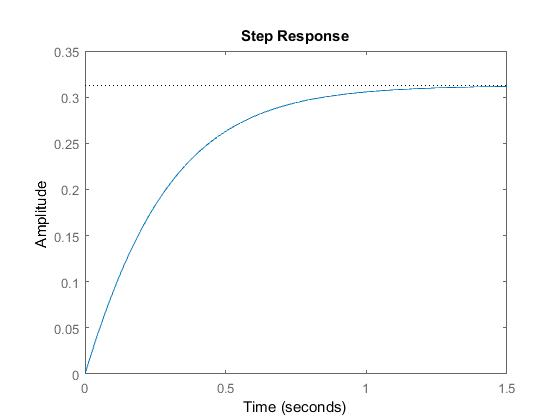
\includegraphics [scale=0.6] {Figures/e21step}
		\end{figure}
		\item Para o impulso unit\'{a}rio, temos:
		\\$Y(s)=\cfrac{s+10}{(s+4)(s+8)}= 
		\cfrac{A}{s+4}+\cfrac{B}{s+8} $
		\begin{itemize}
			\item[o] $A=\lim\limits_{s\to-4}\cfrac{s+10}{s+8}=
			\cfrac{6}{4}\hskip0.7cmB=\lim\limits_{s\to-8}\cfrac{s+10}{s+4}=
			\cfrac{2}{-4}$
		\end{itemize}
		$Y(s)=\cfrac{\cfrac{6}{4}}{s+4}-\cfrac{\cfrac{2}{4}}{s+8}
		\overset{\mathcal{L}^{-1}}{\longrightarrow}
		y(t)=\cfrac{6}{4}e^{-4t}-\cfrac{2}{4}e^{-8t} $
		\begin{figure}[!h]
		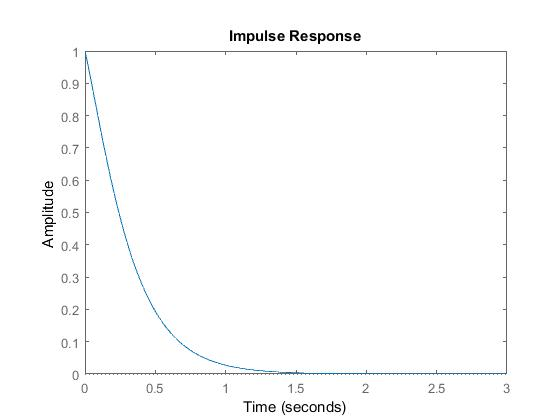
\includegraphics [scale=0.6] {Figures/e21impulse}
		\end{figure}
	\begin{lstlisting}
	%Exercise 2.1
	%Degrau
	syms s
	Y1(s)= (s+10)/(s*(s+4)*(s+8))
	ilaplace(Y1)
	
	num=[1 10];
	den=[1 12 32];
	G=tf(num,den);
	step(G)
	
	%Impulso
	syms s
	Y2(s)= (s+10)/((s+4)*(s+8))
	ilaplace(Y2)
	
	num=[1 10];
	den=[1 12 32];
	G=tf(num,den);
	impulse(G)
	\end{lstlisting}
	\end{itemize}
	\clearpage
	\item Gr\'{a}ficos de $\alpha=[-4, \ -2, \ -1, \ 0, \ 1, \ 2, \ 4]$
	\begin{figure}[!h]
		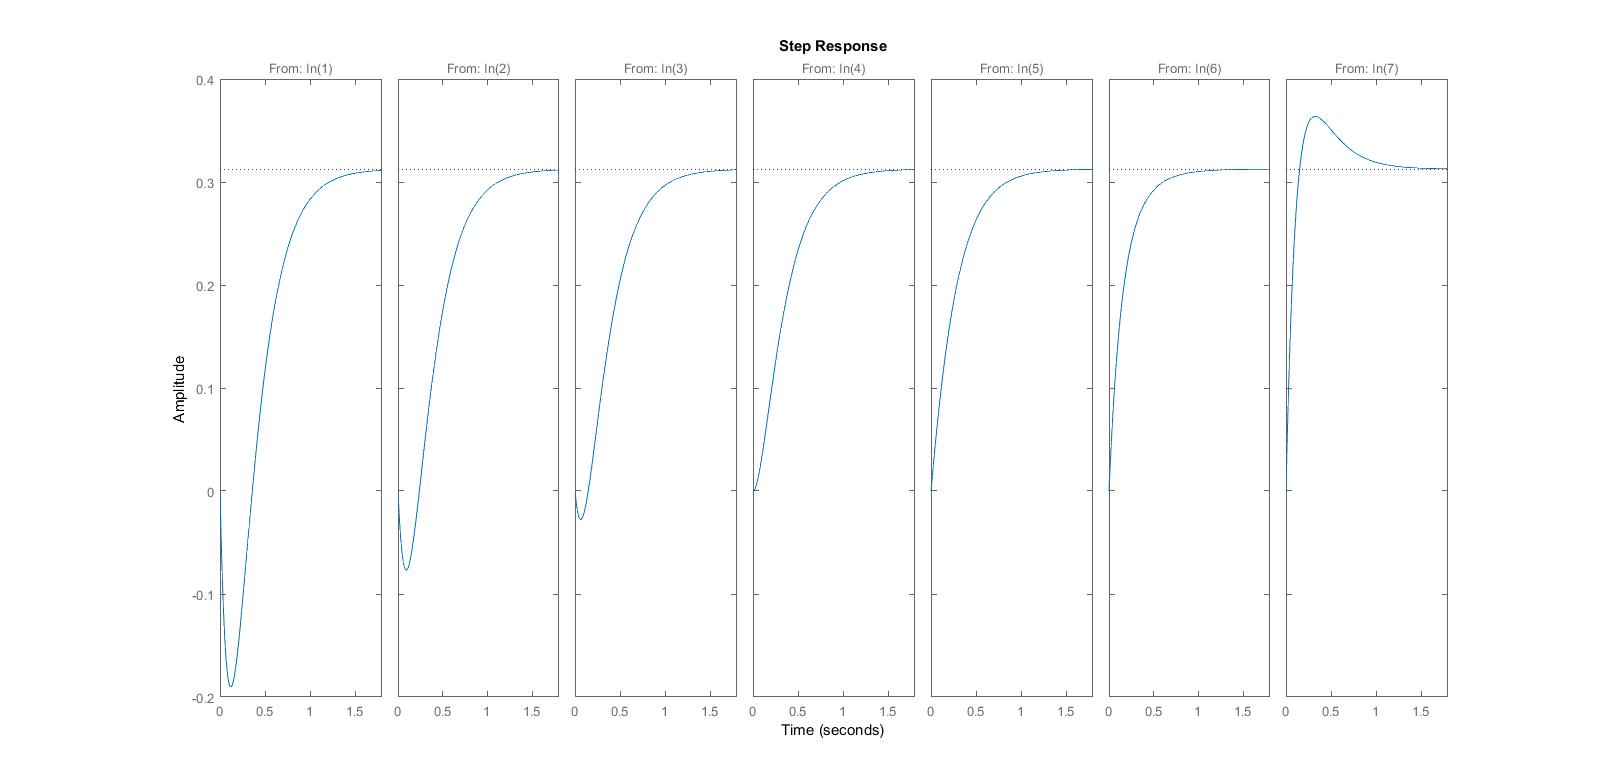
\includegraphics[scale=0.3]{Figures/e22step}
	\end{figure}
	\begin{figure}[!h]
		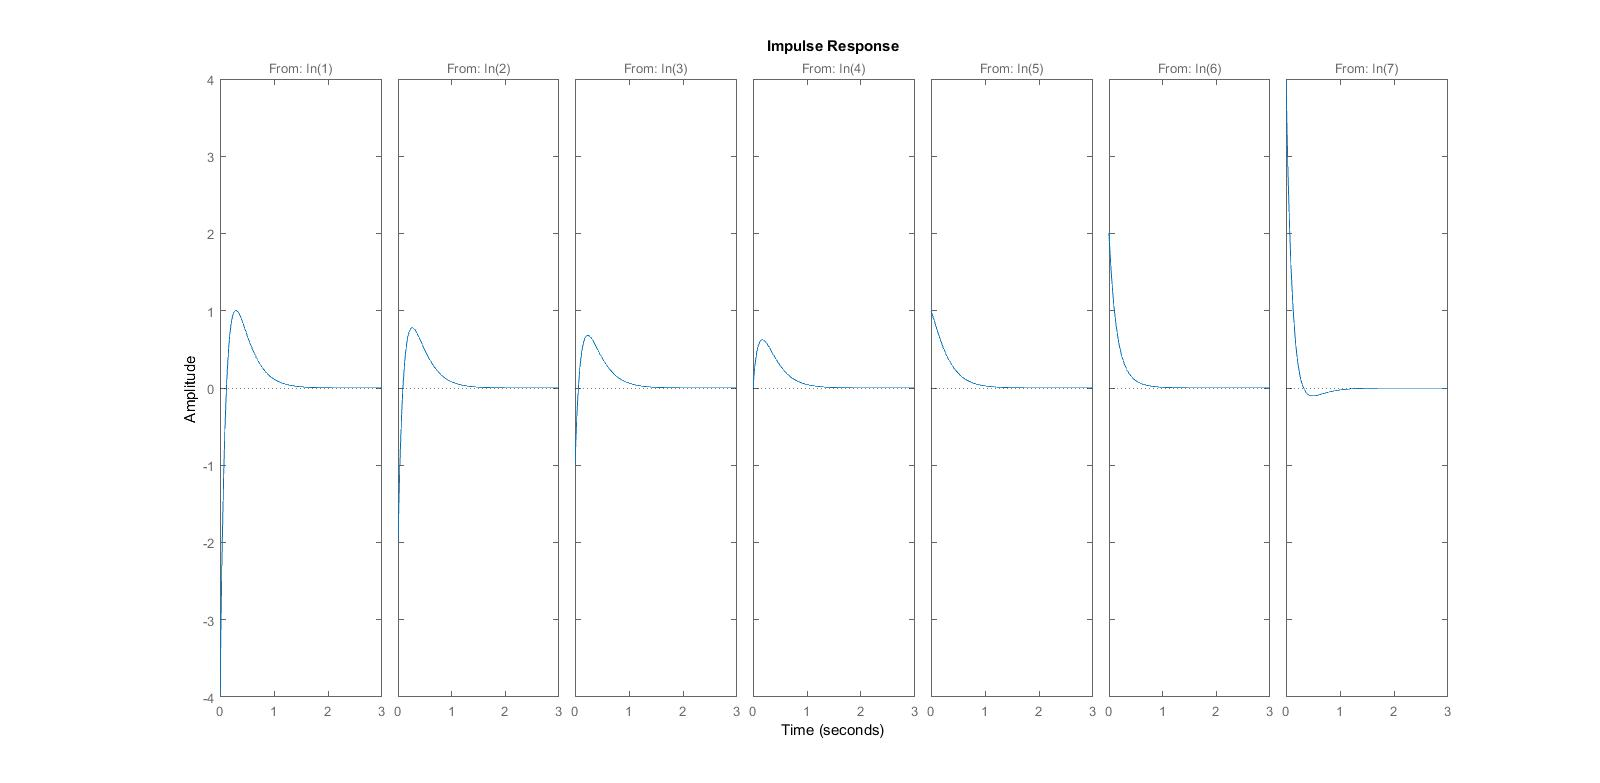
\includegraphics[scale=0.3]{Figures/e22impulse}
	\end{figure}
	\newpage
	\begin{lstlisting}
	%Exercise 2.2
	%degrau
	a = [-4 -2 -1 0 1 2 4]
	for i=1:7
	num=[a(i) 10];
	den=[1 12 32];
	G(i)=tf(num,den);
	end
	step(G)
	
	%impulso
	a = [-4 -2 -1 0 1 2 4]
	for i=1:7
	num=[a(i) 10];
	den=[1 12 32];
	G(i)=tf(num,den);
	end
	impulse(G)
	\end{lstlisting}
	\item Com os gr\'{a}ficos plotados, podemos perceber as situa\c{c}\~{o}es de sobamorte-cimento, sobreamortecimento e amortecimento cr\'{\i}tico. Quando $\alpha=2$, podemos perceber o amortecimento cr\'{\i}tico. Para $\alpha=1$, temos sobreamortecimento. Enquanto para os outros $\alpha$, temos sobamortecimento.
\end{enumerate}
\vskip0.5cm
\section*{Exercise 3} 
Two tanks have cross-sectional areas $S_1$ and $S_2$ [m$^2$], respectively, and are arranged as shown in Figure \ref{fig:ex3}. 
\begin{figure}[ht!]
\begin{center}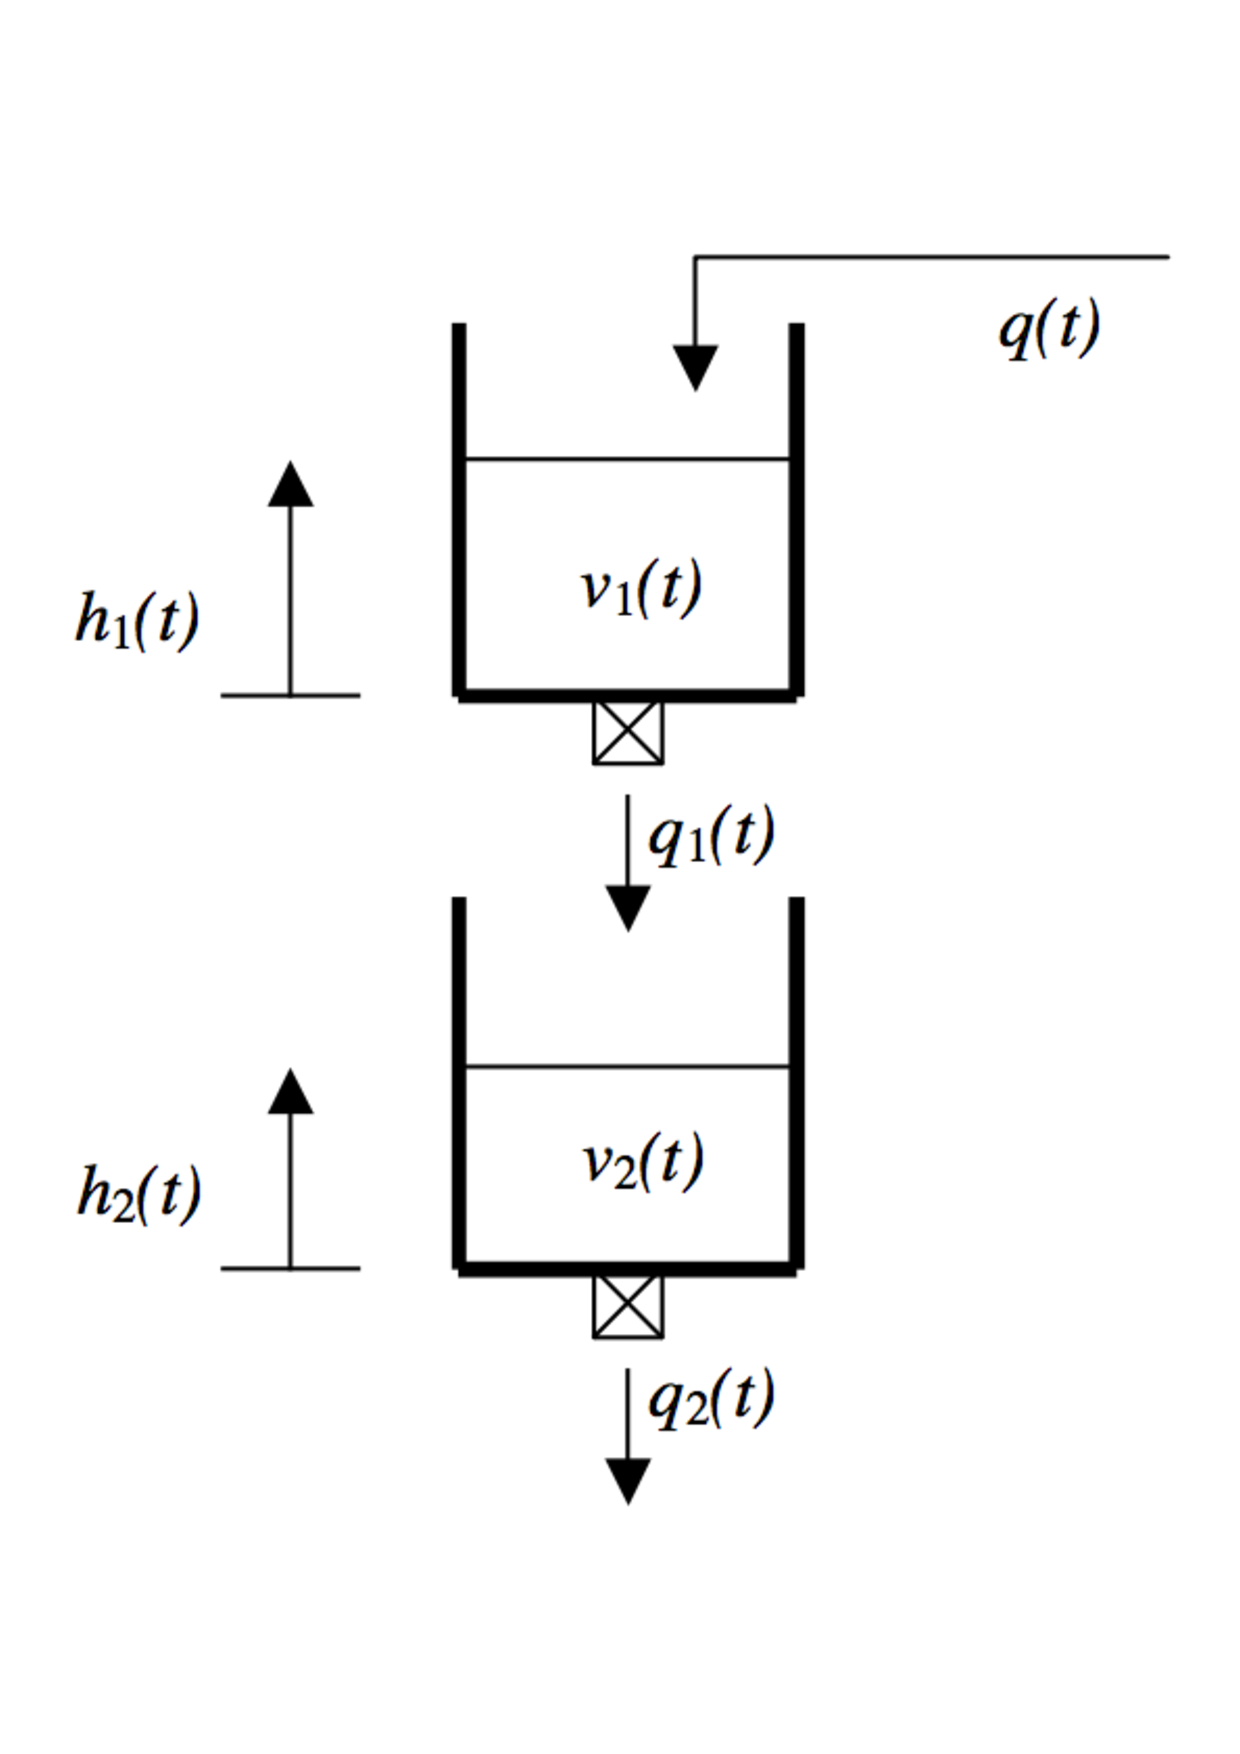
\includegraphics[width=0.44\textwidth]{Figures/tanks_ex} \end{center}
 \vskip-0.5cm\caption{Two-tank system for Exercise 3.}
\label{fig:ex3}
\end{figure}

\noindent The liquid heights on the two tanks are, respectively, $h_1(t)$ and $h_2(t)$ [m] and $v_1(t)$ and $v_2(t)$ are the liquid volumes in the tanks. \\

\noindent The first tank is fed by a flow-rate $q(t)$ [m$^3$/s] and has an output flow-rate given by $q_1(t)=K_1h_1(t)$ [m$^3$/s]. The first tank feeds the second one whose output flow-rate is given by $q_2(t)=K_2h_2(t)$ [m$^3$/s]. The mass conservation law for an incompressible fluid states that the derivatives of the liquid fluid $v(t)$ in the tank is given as
\begin{equation*} 
\cfrac{dv(t)}{dt}=q_{in}(t)-q_{out}(t)
\end{equation*}

\begin{enumerate}
\item Define a state space model for the system where $x_1(t)=v_1(t)$ and $x_2(t)=v_2(t)$ are the state variables, $u(t)=q(t)$ as input and $y(t)=h_2(t)$ as output. 
\item Simulate the state space system, given the following values $S_1=2, \ S_2=4, \ K_1=3, \ K_2=4$ and the following inputs:
\begin{enumerate}
\item A step with amplitude 2 [m$^3$/s] (Hint: Use {\tt stepDataOptions} for modifying the step amplitude). 
\item A square signal with period 5 seconds, duration 30 seconds, and sampling every 0.1 second (Hint: Use {\tt gensig} to generate the input signal).
\end{enumerate}
\item Discuss your results.
\end{enumerate}
\subsection*{Solution 3}
\begin{enumerate}
	\item Temos as seguintes equa\c{c}\~{o}es pelo sistema:
	\begin{itemize}
		\item $\cfrac{dv_1(t)}{dt}=q(t)-q_1(t)=q(t)-K_1h_1(t)$
		\item $\cfrac{dv_2(t)}{dt}=q_1(t)-q_2(t)=K_1h_1(t)-K_2(t)h_2(t) $
		\item $v_1(t)=h_1(t)S_1\rightarrow h_1(t)=\cfrac{v_1(t)}{S_1} $
		\item $v_2(t)=h_2(t)S_2\rightarrow h_2(t)=\cfrac{v_2(t)}{S_2} $
	\end{itemize}
	Substituindo pelas determina\c{c}\~{o}es da quest\~{a}o, temos:
	\\$\dot{x_1}(t)=u(t) -K_1h_1(t)=u(t)-\cfrac{K_1}{S_1}x_1(t) $
	\\$\dot{x_2}(t)=K_1h_1(t)-K_2h_2(t)=
	\cfrac{K_1}{S_1}x_1(t)-	\cfrac{K_2}{S_2}x_2(t)
	\qquad y(t)=\cfrac{x_2(t)}{S_2}$
	\\Com isso, achamos a representa\c{c}\~{a}o em espa\c{c}o de estado:
	\\$\dot{x}=Ax+Bu\rightarrow\dot{x}=
	\begin{bmatrix}
	-\cfrac{K_1}{S_1} & 0\\
	\cfrac{K_1}{S_1} & -\cfrac{K_2}{S_2}
	\end{bmatrix}x+
	\begin{bmatrix}
	1\\
	0
	\end{bmatrix}u$
	\vskip0.4cm
	$y=Cx+Du\rightarrow y=
	\begin{bmatrix}
	0 & \cfrac{1}{S_2}
	\end{bmatrix}q+0u$
	\item Para o degrau:
	\begin{figure}[!h]  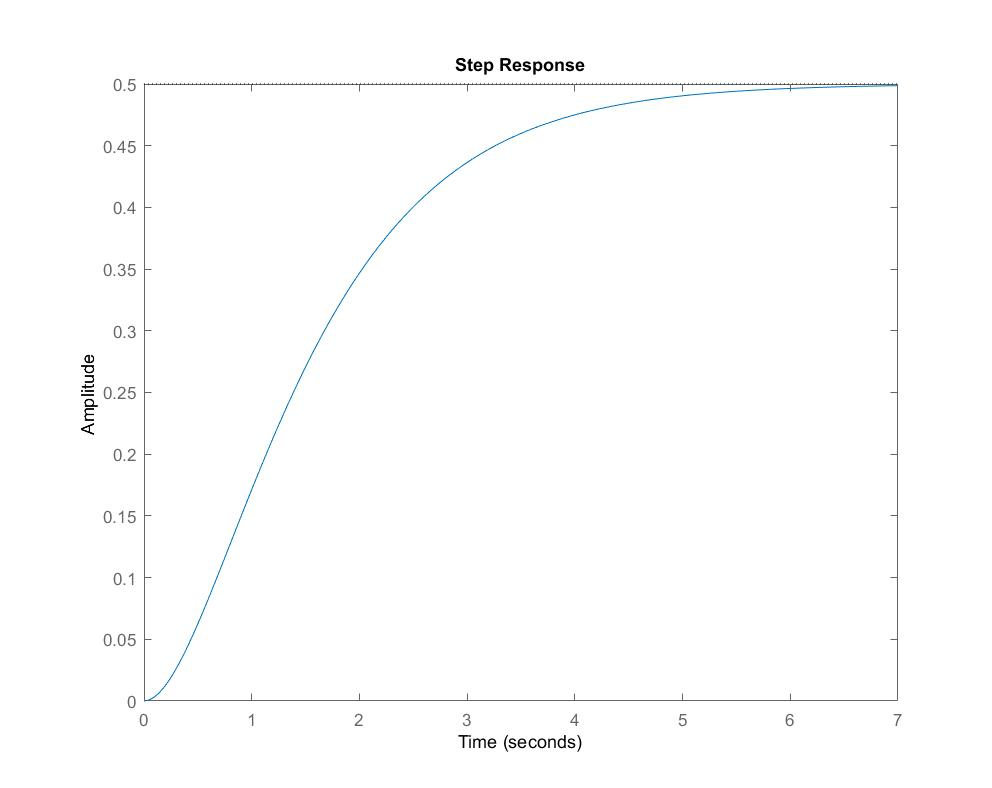
\includegraphics [scale=0.4] {Figures/e32step} \end{figure}
	\begin{lstlisting}
	%Exercise3.2a
	A = [(-3/2) 0;(3/2) (-4/4)];
	B=[1; 0];
	C=[0 (1/4)];
	D=0;
	
	[num,den] = ss2tf(A,B,C,D);
	T = tf(num,den)
	opt = stepDataOptions('StepAmplitude',2);
	step(T,opt)
	\end{lstlisting}
	\begin{figure}[!h]  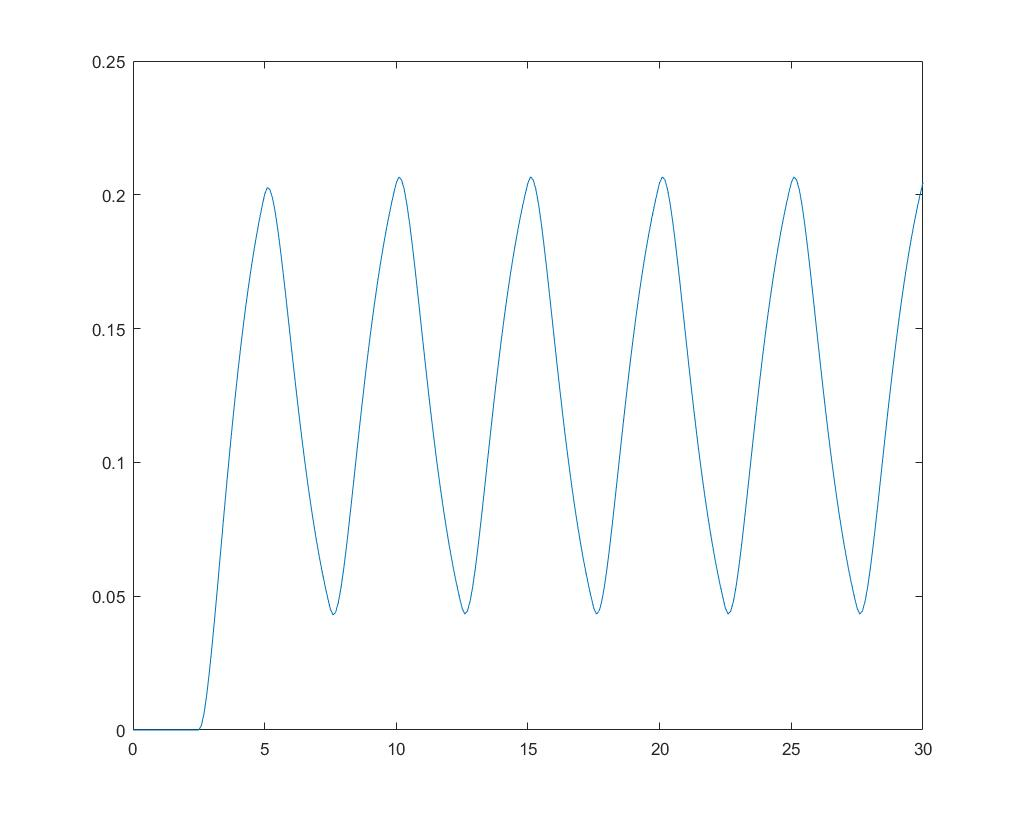
\includegraphics [scale=0.4] {Figures/e32square} \end{figure}
	\begin{lstlisting}
	%Exercise3.2b
	A = [(-3/2) 0;(3/2) (-4/4)];
	B=[1; 0];
	C=[0 (1/4)];
	D=0;
	
	[num,den] = ss2tf(A,B,C,D);
	T = tf(num,den)
	[u,t] = gensig('square',5,30,0.1)
	[y,t]=lsim(T,u,t);
	figure; plot(t,y)
	\end{lstlisting}
\end{enumerate}
\vskip0.5cm
\section*{Exercise 4} 
Given a system described by the IO model in Equation \ref{eq:ex4}:
\begin{equation}
4\ddot{y}(t)+ 7\dot{y}(t)+3y(t)=\ddot{u}(t)+4\dot{u}(t)+4u(t)
\label{eq:ex4}
\end{equation}

\begin{enumerate}
\item Express the system as transfer function $G(s)=Y(s)/U(s)$.
\item Find a state space representation of the system.
\item Verify and comment your results on Matlab/Octave. 
\end{enumerate}
\subsection*{Solution 4}
\begin{enumerate}
	\item $4\ddot{y}(t)+ 7\dot{y}(t)+3y(t)=\ddot{u}(t)+4\dot{u}(t)+4u(t)
	\rightarrow
	\\4s^2Y(s)+7sY(s)+3Y(s)=s^2U(s)+4sU(s)+U(s)
	\rightarrow
	\\Y(s)(4s^2+7s+3)=U(s)(s^2+4s+4)
	\rightarrow$
	\vskip0.4cm
	$G(s)=\cfrac{Y(s)}{U(s)}=\cfrac{s^2+4s+4}{4s^2+7s+3}$
	\item $G(s)=\cfrac{Y(s)}{U(s)}=\cfrac{s^2+4s+4}{4s^2+7s+3}*\cfrac{Z(s)}{Z(s)}\rightarrow$
	\vskip0.4cm
	$Y(s)=(s^2+4s+4)Z(s)
	\overset{\mathcal{L}^{-1}}{\longrightarrow}
	y(t)=\ddot{z}(t)+4\dot{z}(t)+4z(t) $
	\\$U(s)=(4s^2+7s+3)Z(s)
	\overset{\mathcal{L}^{-1}}{\longrightarrow}
	u(t)=4\ddot{z}(t)+7\dot{z}(t)+3z(t) $
	\vskip0.4cm
	Chamando $z(t)=q_1$ e $\dot{z}(t)=q_2$, temos que as vari\'{a}veis de estado s\~{a}o:
	\\$\dot{q_1}=q_2\qquad \qquad \dot{q_2}=\cfrac{1}{4}u(t)-\cfrac{7}{4}q_2-\cfrac{3}{4}q_1$
	\vskip0.4cm
	Achando a sa\'{\i}da:
	\\$y(t)=\ddot{z}(t)+4\dot{z}(t)+4z(t)\rightarrow
	 y(t)=\cfrac{1}{4}u(t)-\cfrac{7}{4}q_2-\cfrac{3}{4}q_1
	 +4q_2+4q_1$
	 \\$y(t)= \cfrac{1}{4}u(t)+\cfrac{9}{4}q_2+\cfrac{13}{4}q_1$
	 \vskip0.4cm
	 Com isso, chegamos a nossa representa\c{c}\~{a}o em espa\c{c}o de estado:\\
	 $\dot{q}=Aq+Bu\rightarrow\dot{q}=
	 \begin{bmatrix}
	 	0 & 1\\
	 	-\cfrac{7}{4} & -\cfrac{3}{4}
	 \end{bmatrix}q+
	 \begin{bmatrix}
	 0\\
	 \cfrac{1}{4}
	 \end{bmatrix}u$
	 \vskip0.4cm
	 $y=Cq+Du\rightarrow y=
	 \begin{bmatrix}
	 \cfrac{13}{4} & \cfrac{9}{4}
	 \end{bmatrix}q+\cfrac{1}{4}u$
	 \newpage
	 \item \begin{lstlisting}
	 %Exercise4.3
	 
	 num=[1 4 4];
	 den=[4 7 3];
	 T=tf(num,den);
	 Tss=ss(T)
	 
	 Tss =
	 
	 A = 
	 x1     x2
	 x1  -1.75  -0.75
	 x2      1      0
	 
	 B = 
	 u1
	 x1   1
	 x2   0
	 
	 C = 
	 x1      x2
	 y1  0.5625  0.8125
	 
	 D = 
	 u1
	 y1  0.25
	 
	 Continuous-time state-space model.
	 \end{lstlisting}
\end{enumerate}
\end{document}